\subsection{Formally smooth algebras}

Let \(k\) be a ring and A a \(k\)-linearly topologized algebra (III, § 4, No. 2, Definition 1).

DEFINITION 1. We say that A is formally smooth over k, or is a formally smooth k-algebra, if it satisfies the following condition: for every k-algebra C and every ideal N of C with square zero, every continuous homomorphism from A to the k-algebra C/N, endowed with the discrete topology, lifts to a continuous homomorphism from A to the k-algebra C, endowed with the discrete topology.

Recall that a homomorphism from A into a \(k\)-algebra equipped with the discrete topology is continuous if and only if its kernel is open.

Let \(k\) be a ring, A a linearly topologized formally smooth \(k\)-algebra, and J an ideal of A. Endow A with the J-adic topology. Let C be a \(k\)-algebra and N an ideal of square zero in C; endow C and C/N with the discrete topology. Let \(\varphi : A \to C/N\) be a continuous homomorphism of algebras. Any lifting \(\tilde{\varphi} : A \to C\) of \(\varphi\) is continuous: indeed, there exists an integer \(n\) such that \(\varphi(J^n)\) is zero, and we have \(\tilde{\varphi}(J^n) \subset N\), whence \(\tilde{\varphi}(J^{2n}) \subset N^2 = 0\). It follows in particular that, if A is formally smooth for the J-adic topology, it is also formally smooth for the J'-adic topology for every ideal J' containing J.

We shall say that a \(k\)-algebra A is formally smooth if it is formally smooth when endowed with the discrete topology, that is, the (0)-adic topology; it is then formally smooth for the J-adic topology for any ideal J of A.

Remarks.- 1) Let \(k\) be a ring, A a linearly topologized formally smooth \(k\)-algebra, and J an ideal of A. If the \(k\)-algebra A/J is formally smooth (for the discrete topology), the identity map of A/J admits a lifting to \(\mathrm{A} / \mathrm{J}^2\); consequently, the sets described in Proposition 2 are nonempty. In particular, the sequence

\[
0 \to J / J ^ {2} \xrightarrow {\bar {d}} (A / J) \otimes_ {A} \Omega_ {k} (A) \longrightarrow \Omega_ {k} (A / J) \to 0
\]

is exact and split.

\begin{enumerate}
\def\labelenumi{\arabic{enumi})}
\setcounter{enumi}{1}
\tightlist
\item
  Let \(k\) be a ring, \(\Lambda\) a formally smooth linearly topologized \(k\)-algebra, M an A-module whose annihilator is open in A. Then every derivation \(\delta\) of \(k\) into M extends to a derivation from A into M. Indeed, set B = A/Ann(M); the map \(\lambda \mapsto (\lambda 1_{B}, \delta(\lambda))\) defines a ring homomorphism from \(k\) into B ⊕ M (No. 1, Example), that is, a structure of \(k\)-algebra on B ⊕ M. The canonical surjection \(\varphi: A \to B\) is continuous, hence admits a lifting \(\tilde{\varphi}: A \to B \oplus M\); according to loc. cit., pr \(_{2}\) \(\circ\) \(\tilde{\varphi}\) is a derivation of \(\Lambda\) into M which extends \(\delta\).
\end{enumerate}

PROPOSITION 3. - Let k be a ring.

\begin{enumerate}
\def\labelenumi{\alph{enumi})}
\item
  Let A and B be linearly topologized k-algebras and \(\mathfrak{p}: \mathrm{A} \to \mathrm{B}\) a continuous homomorphism of k-algebras. If A is formally smooth over \(k\) and B is formally smooth over A, then B is formally smooth over \(k\).
\item
  The product k-algebra of a finite family of formally smooth linearly topologized k-algebras is formally smooth.
\item
  Let A be a \(k\)-linearly topologized algebra, and \(\hat{\Lambda}\) the separated completion of A; for A to be formally smooth over \(k\), it is necessary and sufficient that this be so for \(\hat{\Lambda}\).
\end{enumerate}

Let C be a \(k\)-algebra, A a C-algebra, N an ideal of square zero in C, and \(\pi : \mathrm{C} \to \mathrm{C/N}\) the canonical surjection. Endow C and C/N with the discrete topology.

\begin{enumerate}
\def\labelenumi{\alph{enumi})}
\tightlist
\item
  Let \(\psi : B \to C/N\) be a continuous homomorphism of \(k\)-algebras. Since A is formally smooth over \(k\), there exists a continuous homomorphism of \(k\)-algebras \(\tilde{\varphi} : A \to C\) such that \(\pi \circ \tilde{\varphi} = \psi \circ \rho\).
\end{enumerate}

\pandocbounded{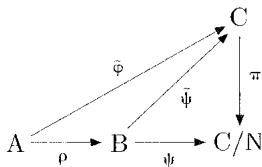
\includegraphics[keepaspectratio]{images/part001_4eedc660.jpg}}

Consider C and C/N as A-algebras by means of \(\tilde{\varphi}\), so that \(\psi\) is a homomorphism of \(A\) -algebras; since B is formally smooth over A, there exists a continuous homomorphism of A-algebras \(\tilde{\psi}: B \to C\) such that \(\pi \circ \tilde{\psi} = \psi\), whence a).

\begin{enumerate}
\def\labelenumi{\alph{enumi})}
\setcounter{enumi}{1}
\item
  It suffices to prove that the product of two formally smooth \(k\)-algebras \(\mathrm{A}_1\) and \(\mathrm{A}_2\) is formally smooth. Let \(\varphi : \mathrm{A}_1 \times \mathrm{A}_2 \to \mathrm{C} / \mathrm{N}\) be a continuous homomorphism of \(k\)-algebras. Set \(e_1 = \varphi(1,0)\), \(e_2 = \varphi(0,1)\), so that \(e_1\) and \(e_2\) are orthogonal idempotents in \(\mathrm{C} / \mathrm{N}\). Let \(\varphi_1 : \mathrm{A}_1 \to (\mathrm{C} / \mathrm{N})e_1\) and \(\varphi_2 : \mathrm{A}_2 \to (\mathrm{C} / \mathrm{N})e_2\) be the maps defined by \(\varphi_1(a_1) = \varphi(a_1,0)\) and \(\varphi_2(a_2) = \varphi(0,a_2)\); these are continuous homomorphisms of \(k\)-algebras, and one has \(\varphi(a_1,a_2) = \varphi_1(a_1) + \varphi_2(a_2)\) for every \((a_1,a_2) \in \mathrm{A}_1 \times \mathrm{A}_2\). There exists an idempotent element \(\tilde{e}_1\) of C such that \(\pi(\tilde{e}_1) = e_1\) (A, VIII, § 9, No. 4, Proposition 7); set \(\tilde{e}_2 = 1 - \tilde{e}_1\), so that \(\pi(\tilde{e}_2) = e_2\). To show that this holds for \(i = 1,2\), the homomorphism \(\mathrm{C}\tilde{e}_i \to (\mathrm{C} / \mathrm{N})e_i\) induced by \(\pi\) is surjective, with kernel \(\mathrm{N}\tilde{e}_i\); since the \(k\)-algebra \(\mathrm{A}_i\) is formally smooth, the homomorphism \(\varphi_i\) admits a continuous lifting \(\tilde{\varphi}_i\) to \(\mathrm{C}\tilde{e}_i\). The map \((a_1,a_2) \mapsto \tilde{\varphi}_1(a_1) + \tilde{\varphi}_2(a_2)\) is a continuous lifting of \(\varphi\) to C.
\item
  Let \(i: \mathrm{A} \to \widehat{\mathrm{A}}\) be the canonical homomorphism. For every ring D equipped with the discrete topology, the map that assigns to a continuous homomorphism \(f: \widehat{\mathrm{A}} \to \mathrm{D}\) the continuous homomorphism \(f \circ i: \mathrm{A} \to \mathrm{D}\) is bijective. Assertion c) follows from this.
\end{enumerate}

The assertion c) of the proposition applies in particular when the topology of \(A\) is the J-adic topology, where \(J\) is a finitely generated ideal: the closure \(\widehat{J}\) of \(J\) in \(\widehat{A}\) is then equal to \(\widehat{JA}\) and the topology of \(\widehat{A}\) is the topology \(\widehat{J}\)-adic (III, § 2, No. 12, Corollary 2 of Proposition 16). Consequently, it is equivalent to say that \(A\) is formally smooth for the J-adic topology or that its separated completion \(\widehat{A}\) is formally smooth for the J-adic topology.

PROPOSITION 4.--- Let k be a ring, A and B k-algebras, J an ideal of A, and K an ideal of B.

\begin{enumerate}
\def\labelenumi{\alph{enumi})}
\item
  Let S be a multiplicative subset of A and T a subset of k whose image in A is contained in S. If \(A\) is formally smooth over \(k\) for the J-adic topology, S \(^{-1}A\) is formally smooth over \(\mathrm{T}^{-1}k\) for the topology \(\mathrm{S}^{-1}\mathrm{J}\)-adic.
\item
  Let \(k'\) be a \(k\)-algebra. If A is formally smooth over \(k\) for the J-adic topology, the \(k'\)-algebra \(A_{(k')}\) is formally smooth over \(k'\) for the \(JA_{(k')}\)-adic topology.
\item
  Let I denote the ideal of A ⊗k B generated by the images of J ⊗k B and A ⊗k K. If A and B are formally smooth over k for the J-adic and K-adic topologies, respectively, then the k-algebra A ⊗k B is formally smooth for the I-adic topology.
\item
  Under the hypotheses of a), let C be a \(\mathrm{T}^{-1}k\)-algebra and N an ideal of square zero in C; endow C and C/N with the discrete topology and denote \(\pi : C \to C/N\) the canonical surjection. Let \(\varphi : S^{-1}A \longrightarrow C/N\) be a homomorphism of \(\mathrm{T}^{-1}k\)-algebras, continuous for the \(\mathrm{S}^{-1}\mathrm{J}\)-adic topology. Denote by i the canonical homomorphism from A into \(S^{-1}A\). The map \(\varphi \circ i\) is a homomorphism of k-algebras, continuous for the J-adic topology, hence admits a lifting \(\tilde{\varphi}_{0} : A \to C\). The elements of \(\tilde{\varphi}_{0}(S)\) are invertible modulo N, hence invertible since N is nilpotent. Consequently there exists a ring homomorphism \(\tilde{\varphi} : S^{-1}A \to C\) such that \(\tilde{\varphi} \circ i = \tilde{\varphi}_{0}\) (II, § 2, No. 1, Proposition 1); by Corollary 3 of Proposition 2 of loc. cit., \(\tilde{\varphi}\) is \(\mathrm{T}^{-1}k\)-linear. We have \(\pi \circ \tilde{\varphi} \circ i = \varphi \circ i\), whence \(\pi \circ \tilde{\varphi} = \varphi\) (loc. cit., Proposition 1), so that \(\tilde{\varphi}\) is a lifting of \(\varphi\).
\item
  Let us place ourselves under the hypotheses of b). Let C be a \(k'\)-algebra and N an ideal of square zero in C; endow C and C/N with the discrete topology. Let \(\varphi : \mathrm{A}_{(k')} \longrightarrow \mathrm{C/N}\) be a homomorphism of \(k'\)-algebras, continuous for the \(J\mathrm{A}_{(k')}\)-adic topology. Let \(i : \mathrm{A} \to \mathrm{A}_{(k')}\) denote the canonical homomorphism. The map \(\varphi \circ i\) is a homomorphism of \(k\)-algebras from A to C/N, continuous for the J-adic topology; if A is formally smooth over \(k\) for the J-adic topology, \(\varphi \circ i\) admits a lifting \(\tilde{\psi} : \mathrm{A} \to \mathrm{C}\). The homomorphism of \(k'\)-algebras \(\tilde{\varphi} : \mathrm{A}_{(k')} \longrightarrow \mathrm{C}\) deduced from \(\tilde{\psi}\) is a lifting of \(\varphi\).
\item
  We place ourselves under the hypotheses of c). The B-algebra A⊗ \(_{k}\) B is formally smooth for the J(A⊗ \(_{k}\) B)-adic topology by b), hence for the I-adic topology; moreover, the canonical homomorphism B → A⊗ \(_{k}\) B is continuous when B is equipped with the K-adic topology and A⊗ \(_{k}\) B with the I-adic topology. Assertion c) therefore follows from Proposition 3, a).
\end{enumerate}

